\chapter{Fundamenta\c{c}\~ao Te\'orica - Revis\~ao Bibliogr\'afica}
\label{cap:fundamentacao}

\section{Experimenta\c{c}\~ao agr\'icola, parcelas experimentais e fenotipagem vegetal}
\label{sec:experimentacao-agricola}

A experimenta\c{c}\~ao de campo subdivide a \'area dispon\'ivel em parcelas \`as quais se associam tratamentos ou materiais gen\'eticos, possibilitando relacionar observa\c{c}\~oes (biomassa, altura, cobertura vegetal) \`a unidade experimental correspondente. Por isso, al\'em de regi\~ao f\'isica cultivada, a parcela possui uma identidade dentro da estrutura do experimento: uma informa\c{c}\~ao perde parte de sua utilidade quando n\~ao \'e poss\'ivel determinar de qual unidade ela foi obtida. Essa organiza\c{c}\~ao pode ser registrada em croquis que representam posi\c{c}\~oes e, quando dispon\'iveis, identificadores das unidades experimentais, frequentemente segundo um padr\~ao de linhas e colunas.

\begin{figure}[htb]
  \centering
  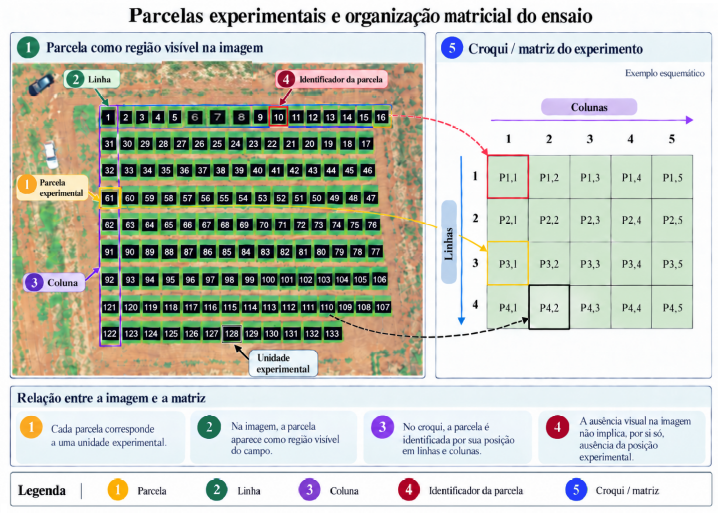
\includegraphics[width=0.9\textwidth]{figuras/figura03.png}
  \caption{Representa\c{c}\~ao da organiza\c{c}\~ao matricial de parcelas experimentais em ortomosaico obtido por drone.}
  \label{fig:organizacao-matricial}
  \fonte{Elaborado pelo autor (2026).}
\end{figure}

A fenotipagem vegetal compreende a obten\c{c}\~ao e an\'alise de caracter\'isticas observ\'aveis resultantes da intera\c{c}\~ao entre componentes gen\'eticos e condi\c{c}\~oes ambientais. Quando o n\'umero de materiais avaliados cresce, a quantidade de observa\c{c}\~oes necess\'arias cresce na mesma propor\c{c}\~ao, configurando um dos problemas reconhecidos para aproveitar plenamente os avan\c{c}os da gen\'etica e do melhoramento de plantas \citep{araus2014}. A fenotipagem de alto rendimento, ou \textit{high-throughput phenotyping}, designa o conjunto de estrat\'egias que responde a esse problema pela integra\c{c}\~ao de sensores, plataformas de aquisi\c{c}\~ao e m\'etodos computacionais, ampliando a escala e a velocidade com que as caracter\'isticas s\~ao registradas. Seu prop\'osito n\~ao \'e substituir as avalia\c{c}\~oes convencionais, mas aumentar a quantidade, a frequ\^encia ou a objetividade das observa\c{c}\~oes poss\'iveis em campo.

Para a an\'alise computacional de imagens, essa organiza\c{c}\~ao espacial \'e o que distingue duas representa\c{c}\~oes do mesmo experimento: a estrutura previamente definida no planejamento de campo e aquilo que pode ser efetivamente observado na imagem. Assim, a parcela deve ser compreendida simultaneamente como regi\~ao vis\'ivel e como posi\c{c}\~ao pertencente \`a organiza\c{c}\~ao espacial do ensaio, distin\c{c}\~ao que se tornar\'a central adiante, ao explicar por que uma aus\^encia visual n\~ao implica, necessariamente, que a posi\c{c}\~ao experimental correspondente deixou de existir.

\section{Sensoriamento remoto e aquisi\c{c}\~ao de imagens orbitais e de drone}
\label{sec:sensoriamento-remoto}

O sensoriamento remoto consiste na obten\c{c}\~ao de informa\c{c}\~oes sobre um alvo sem contato f\'isico direto com ele. Na an\'alise agr\'icola, sensores instalados em plataformas terrestres, a\'ereas ou orbitais permitem registrar propriedades da superf\'icie e da vegeta\c{c}\~ao a partir da radia\c{c}\~ao eletromagn\'etica refletida ou emitida.

Entre os sensores utilizados em aplica\c{c}\~oes agr\'icolas est\~ao as c\^ameras que operam na regi\~ao vis\'ivel do espectro e produzem imagens RGB. Essas imagens registram a intensidade da luz nas bandas correspondentes ao vermelho (RED), verde (GREEN) e azul (BLUE) e podem fornecer informa\c{c}\~oes relacionadas \`a estrutura aparente, cobertura e distribui\c{c}\~ao espacial da vegeta\c{c}\~ao.

Imagens de sat\'elite permitem observar extensas \'areas da superf\'icie em diferentes momentos, com caracter\'isticas de resolu\c{c}\~ao espacial, temporal e espectral que dependem do sensor e do produto disponibilizado. Para a identifica\c{c}\~ao de parcelas experimentais, a adequa\c{c}\~ao dessas imagens depende especialmente da rela\c{c}\~ao entre a resolu\c{c}\~ao espacial e o tamanho f\'isico das unidades que se pretende distinguir.

Em plataformas a\'ereas de baixa altitude, como drones, a combina\c{c}\~ao de m\'ultiplas fotografias pode produzir um ortomosaico, isto \'e, uma representa\c{c}\~ao cont\'inua da \'area constru\'ida a partir de m\'ultiplas imagens corrigidas e geometricamente combinadas. A utiliza\c{c}\~ao de ortomosaicos facilita a an\'alise de uma \'area experimental como uma \'unica superf\'icie visual, embora o processo de constru\c{c}\~ao possa introduzir distor\c{c}\~oes locais. \citet{mardanisamani2021}, por exemplo, observam que a forma\c{c}\~ao do ortomosaico a partir de v\'arias imagens pode produzir deforma\c{c}\~oes que dificultam o alinhamento preciso das micro parcelas com a estrutura te\'orica do campo.

Imagens orbitais oferecem uma rela\c{c}\~ao diferente entre cobertura, frequ\^encia e resolu\c{c}\~ao espacial em compara\c{c}\~ao a plataformas a\'ereas de baixa altitude; a adequa\c{c}\~ao de uma imagem para identificar parcelas individuais depende desta resolu\c{c}\~ao e do tamanho f\'isico das unidades experimentais, n\~ao apenas da origem do sensor. Foram utilizadas imagens orbitais, incluindo registros hist\'oricos disponibilizados pelo Google Earth, e ortomosaicos obtidos por drone em campos experimentais da Embrapa Gado de Corte.

\begin{figure}[htb]
  \centering
  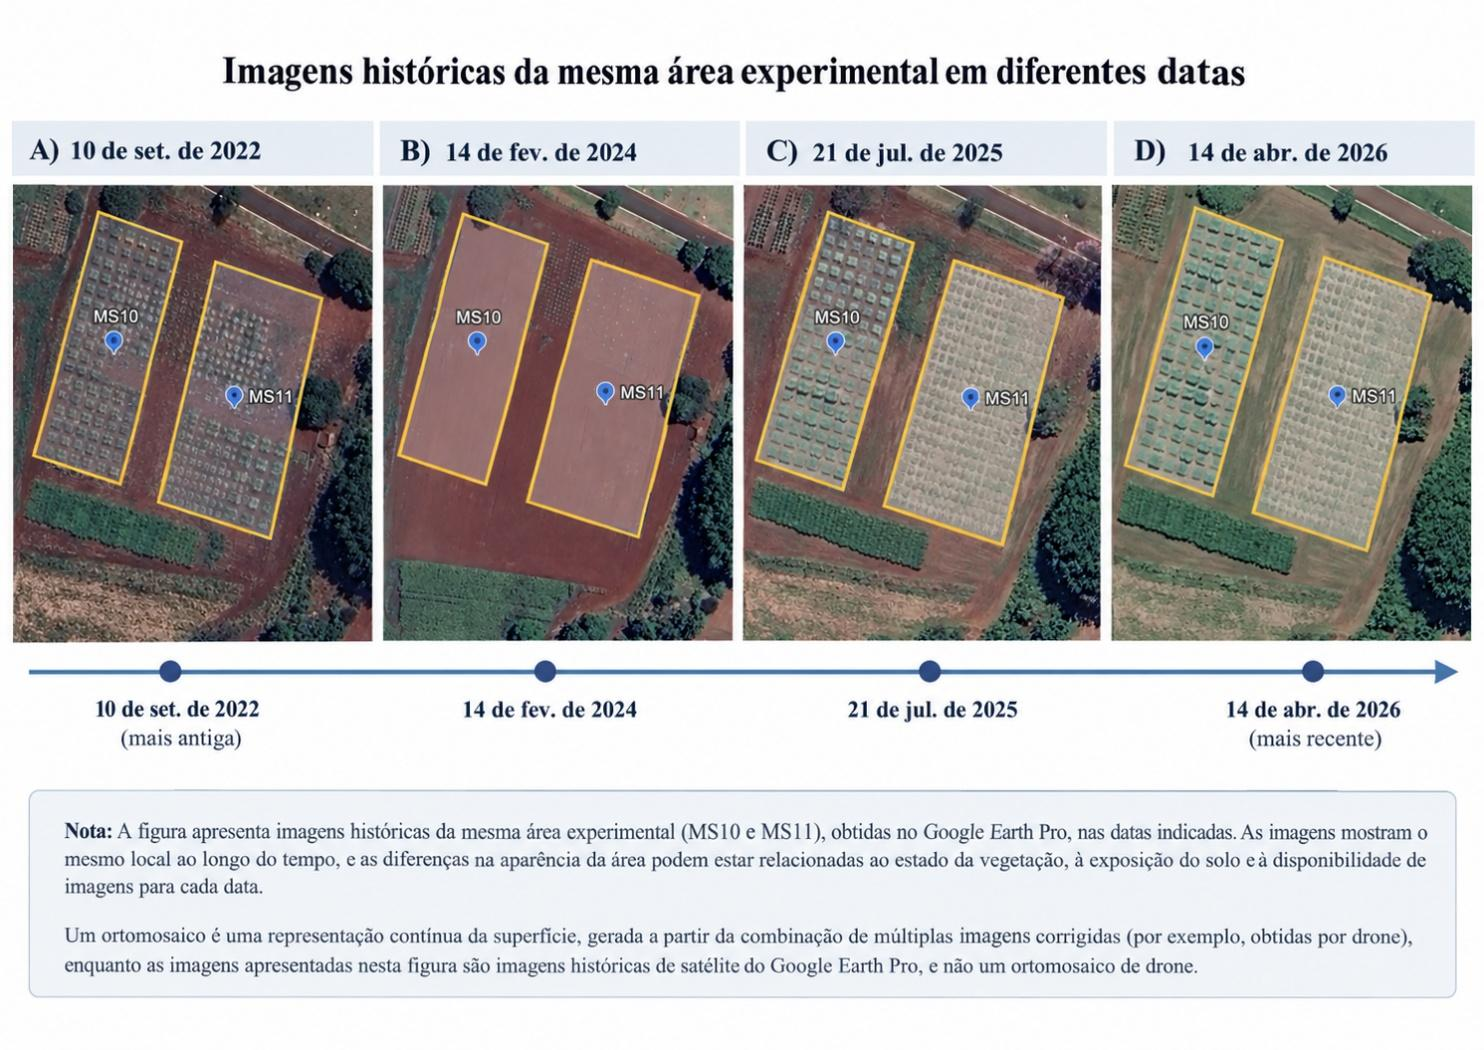
\includegraphics[width=0.95\textwidth]{figuras/figura04.jpg}
  \caption{Imagens hist\'oricas de sat\'elite da mesma \'area experimental em diferentes datas.}
  \label{fig:imagens-historicas}
  \fonte{Google Earth Pro, imagens hist\'oricas do ponto 20\textdegree 26'43.76"S, 54\textdegree 43'11.38"W. Elabora\c{c}\~ao do autor.}
\end{figure}

\section{Resolu\c{c}\~ao espacial e \textit{Ground Sample Distance}}
\label{sec:resolucao-espacial}

A resolu\c{c}\~ao espacial descreve o n\'ivel de detalhe representado por uma imagem, isto \'e, a menor extens\~ao do terreno que pode ser distinguida em seus elementos. Em dados obtidos por sensores digitais, uma maneira de expressar essa rela\c{c}\~ao \'e por meio da Dist\^ancia de Amostragem do Solo, ou \textit{\textbf{Ground Sample Distance} (GSD)}, que representa a dimens\~ao f\'isica do terreno correspondente \`a dist\^ancia entre pixels adjacentes na imagem.

Um pixel \'e o menor elemento que comp\~oe uma imagem digital, ao qual se associa um valor de intensidade ou de cor. Um GSD menor indica que cada pixel corresponde a uma extens\~ao menor da superf\'icie e, portanto, que detalhes espaciais menores podem ser representados na imagem. A capacidade efetiva de distinguir determinado objeto, contudo, tamb\'em depende de outras caracter\'isticas da aquisi\c{c}\~ao, do sensor, da qualidade da imagem e das propriedades visuais do pr\'oprio alvo.

\begin{figure}[htb]
  \centering
  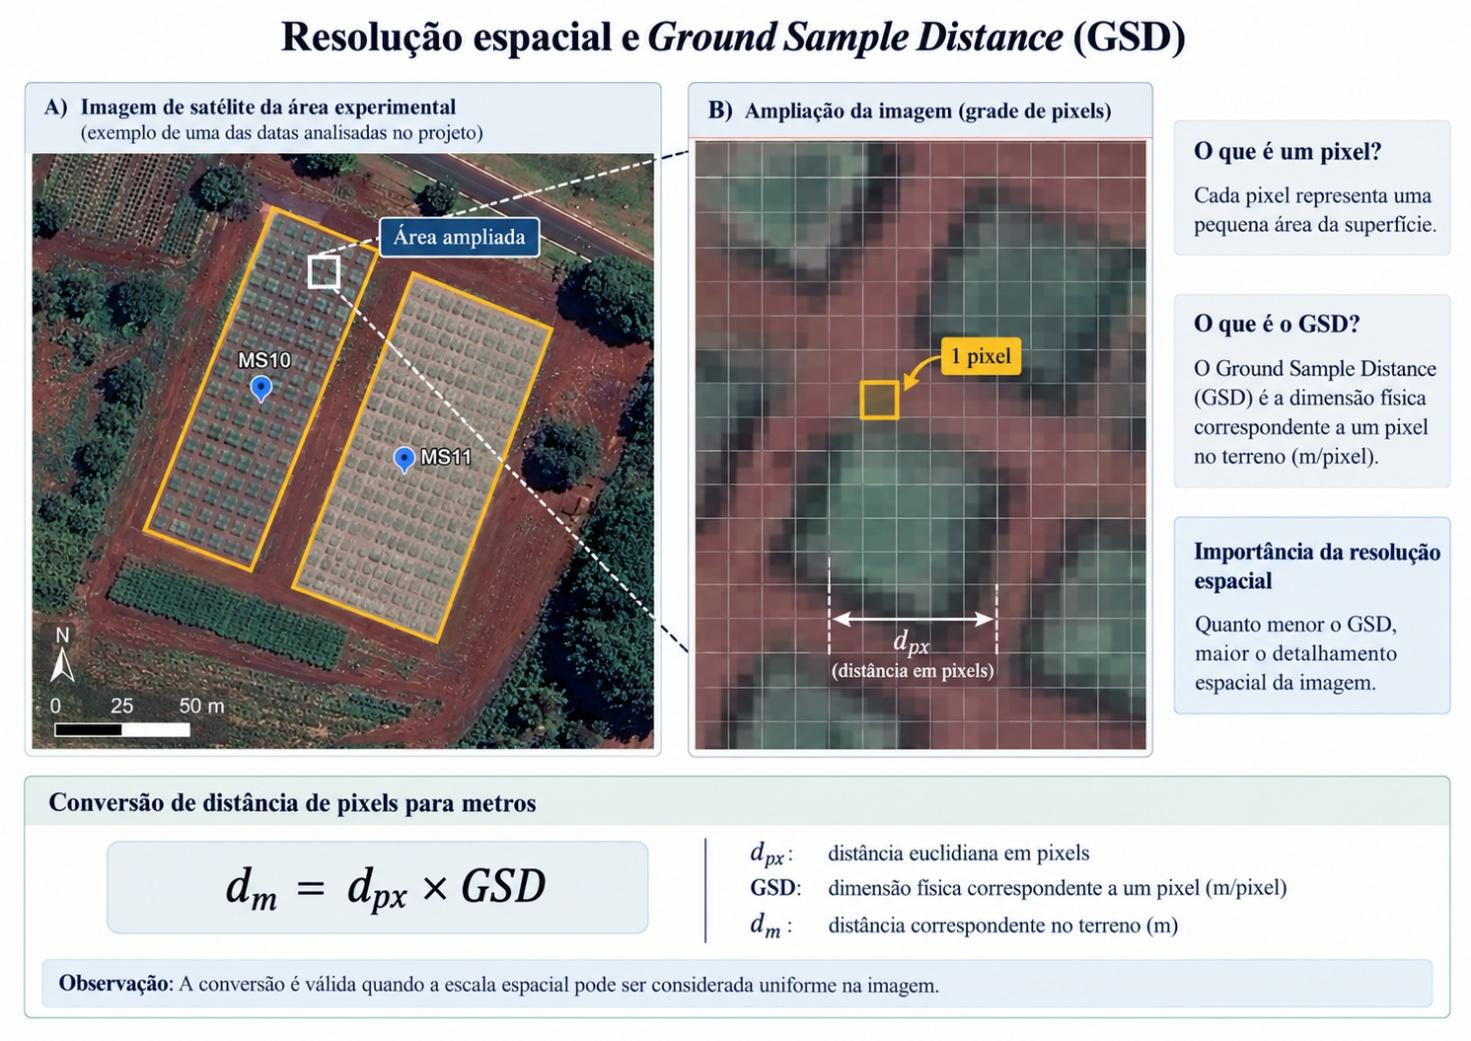
\includegraphics[width=0.9\textwidth]{figuras/figura05.jpg}
  \caption{Rela\c{c}\~ao entre resolu\c{c}\~ao espacial, pixel e Ground Sample Distance (GSD) em imagem de sat\'elite da \'area experimental.}
  \label{fig:gsd}
  \fonte{Elaborado pelo autor (2026).}
\end{figure}

O GSD pode ser utilizado para converter dist\^ancias em pixels para unidades f\'isicas quando a escala for conhecida e aplic\'avel \`a imagem medida. Sob a hip\'otese de uma escala espacial uniforme e igual nos dois eixos, se $d_{px}$ representa a dist\^ancia euclidiana em pixels e o GSD est\'a expresso em metros por pixel, obt\'em-se

\begin{equation}
  d_m = d_{px} \cdot \mathit{GSD}
  \label{eq:gsd}
\end{equation}

em que $d_m$ representa a dist\^ancia em metros.

Na implementa\c{c}\~ao do projeto, o GSD \'e tratado em metros por pixel e pode ser usado para converter dist\^ancias entre centros, em pixels, para metros.

No contexto deste trabalho, o GSD n\~ao \'e assumido como uma vari\'avel experimental cuja influ\^encia j\'a tenha sido sistematicamente avaliada. Sua import\^ancia est\'a principalmente na interpreta\c{c}\~ao espacial das medidas produzidas pelo sistema.

\section{Vis\~ao computacional, representa\c{c}\~ao de objetos e aprendizagem profunda (\textit{deep learning})}
\label{sec:visao-computacional}

A vis\~ao computacional formula diferentes tarefas a partir da mesma imagem, distinguindo-se pela natureza e pela precis\~ao da informa\c{c}\~ao produzida. Na classifica\c{c}\~ao, associa-se um r\'otulo ao conte\'udo global da imagem; na detec\c{c}\~ao, cada inst\^ancia \'e associada a uma classe e a uma regi\~ao espacial, geralmente uma caixa delimitadora; na segmenta\c{c}\~ao de inst\^ancias, acrescenta-se uma m\'ascara por objeto, isto \'e, um conjunto de pixels marcados como pertencentes \`aquele objeto espec\'ifico, o que distingue indiv\'iduos de uma mesma classe. O \textbf{Mask R-CNN}, arquitetura que estende um detector de duas etapas com um ramo dedicado \`a predi\c{c}\~ao dessas m\'ascaras, \'e um exemplo consolidado dessa formula\c{c}\~ao, realizando detec\c{c}\~ao e segmenta\c{c}\~ao simultaneamente \citep{he2017}. Em sentido mais amplo, a localiza\c{c}\~ao de um objeto pode ainda ser reduzida a um conjunto de pontos ou a uma posi\c{c}\~ao pontual, utilizada nesta pesquisa para sintetizar a localiza\c{c}\~ao de uma parcela.

Essa separa\c{c}\~ao \'e crucial, pois a caixa delimitadora, a m\'ascara de segmenta\c{c}\~ao e a representa\c{c}\~ao por ponto oferecem distintas granularidades de dados. Enquanto a caixa define a \'area espacial de forma resumida, a m\'ascara detalha a regi\~ao pixel a pixel, e o ponto apenas indica a posi\c{c}\~ao, sem capturar a forma ou o tamanho. N\~ao existe uma abordagem intrinsecamente melhor que as outras; a escolha ideal reside na aplica\c{c}\~ao espec\'ifica que se pretende executar.

Redes Neurais Convolucionais (\textbf{CNN}) aprendem representa\c{c}\~oes a partir dos dados. O treinamento utiliza uma fun\c{c}\~ao de perda, \textit{loss}, que quantifica a discrep\^ancia entre a sa\'ida produzida e a resposta esperada. A retropropaga\c{c}\~ao aplica a regra da cadeia para calcular os gradientes dessa perda em rela\c{c}\~ao aos par\^ametros da rede; o otimizador utiliza essas informa\c{c}\~oes para atualizar os par\^ametros \citep{pytorch2024}. Essa capacidade, por\'em, n\~ao garante robustez a condi\c{c}\~oes representadas no treinamento: a generaliza\c{c}\~ao precisa ser avaliada sobre dados suficientemente independentes daqueles usados no ajuste do modelo.

Uma caixa horizontal (\textit{\textbf{Horizontal Bounding Box}, HBB}) permanece alinhada aos eixos da imagem e pode ser descrita por

\begin{equation}
  b_{HBB} = \left(x_c, y_c, w, h\right)
  \label{eq:hbb}
\end{equation}

onde $x_c$ e $y_c$ s\~ao as coordenadas do centro e $w$ e $h$ s\~ao largura e altura.

Quando o objeto tem orienta\c{c}\~ao distinta da dos eixos, essa representa\c{c}\~ao pode incluir uma quantidade maior de regi\~ao externa ao objeto. A \textit{\textbf{Oriented Bounding Box} (OBB)} acrescenta a orienta\c{c}\~ao:

\begin{equation}
  b_{OBB} = \left(x_c, y_c, w, h, \theta\right)
  \label{eq:obb}
\end{equation}

reduzindo essa regi\~ao externa para objetos rotacionados, situa\c{c}\~ao particularmente estudada em imagens a\'ereas de alta densidade \citep{ding2019}. Essa propriedade geom\'etrica n\~ao implica que a OBB seja necessariamente superior \`a HBB ou \`a segmenta\c{c}\~ao de inst\^ancias.

\begin{figure}[htb]
  \centering
  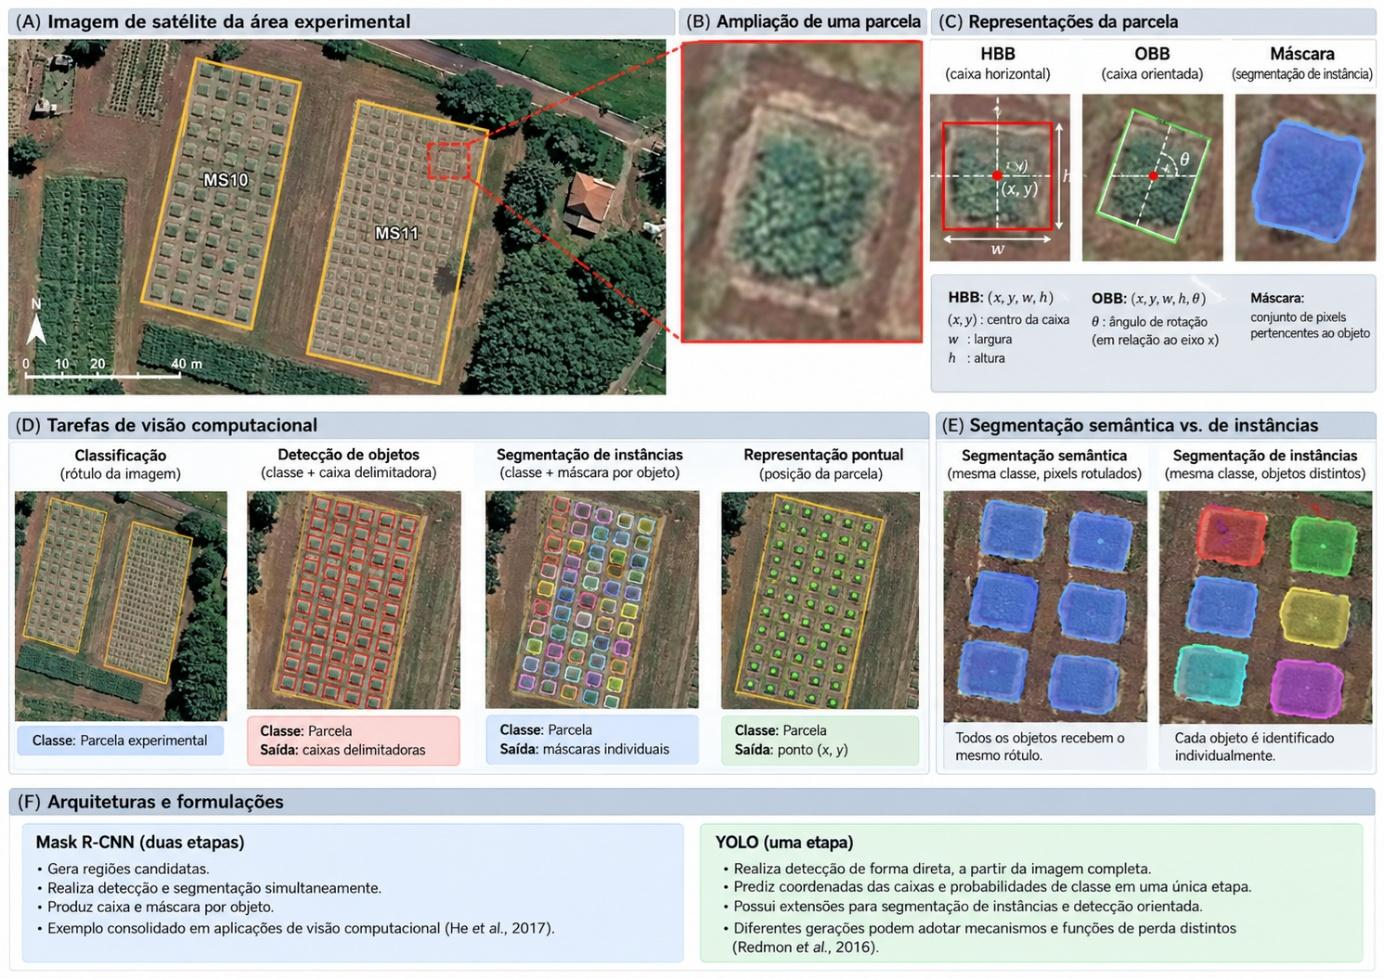
\includegraphics[width=0.95\textwidth]{figuras/figura06.jpg}
  \caption{Representa\c{c}\~oes de objetos em vis\~ao computacional aplicadas \`a identifica\c{c}\~ao de parcelas experimentais em imagens orbitais.}
  \label{fig:representacoes-objetos}
  \fonte{Elaborado pelo autor (2026).}
\end{figure}

Na segmenta\c{c}\~ao sem\^antica, pixels da mesma categoria recebem o mesmo r\'otulo independentemente de pertencerem a objetos fisicamente distintos; a segmenta\c{c}\~ao de inst\^ancias preserva, al\'em da categoria, a identidade individual de cada objeto. Essa distin\c{c}\~ao \'e relevante para experimentos agr\'icolas em que todas as parcelas compartilham uma mesma classe sem\^antica, mas ainda precisam ser contadas e manipuladas individualmente. No conjunto de 277 imagens, as parcelas foram anotadas como quadril\'ateros sob uma \'unica classe; outras organiza\c{c}\~oes dos dados usam anota\c{c}\~oes poligonais ou pontuais.

O \textbf{\textit{YOLO} (\textit{You Only Look Once})} \'e uma fam\'ilia de detectores de est\'agio \'unicos, proposta originalmente por \citet{redmon2016}. Sua formula\c{c}\~ao trata a detec\c{c}\~ao como um problema de regress\~ao direta, isto \'e, a rede prediz de uma s\'o vez, a partir da imagem completa, as coordenadas das caixas e as probabilidades de classe, sem uma etapa separada de gera\c{c}\~ao de regi\~oes candidatas seguida de classifica\c{c}\~ao, como faziam abordagens anteriores. Tal formula\c{c}\~ao deu origem a uma fam\'ilia posteriormente estendida a segmenta\c{c}\~ao de inst\^ancias e detec\c{c}\~ao orientada. N\~ao \'e adequado, contudo, assumir que todas as gera\c{c}\~oes compartilham a mesma arquitetura interna ou diferem apenas em profundidade ou n\'umero de par\^ametros: cada gera\c{c}\~ao pode alterar mecanismos de extra\c{c}\~ao e fus\~ao de caracter\'isticas, fun\c{c}\~oes de perda e estrat\'egias de atribui\c{c}\~ao. Por isso, os experimentos hist\'oricos do projeto com diferentes vers\~oes de YOLO n\~ao s\~ao assumidos de forma que possam ser diretamente compar\'aveis apenas por pertencerem \`a mesma fam\'ilia.

\section{Centros, centroides e representa\c{c}\~ao espacial}
\label{sec:centros-centroides}

Uma representa\c{c}\~ao bidimensional complexa pode ser sintetizada por meio de um ponto que indique sua posi\c{c}\~ao central. Conv\'em, por\'em, identificar sobre quais elementos esse ponto \'e calculado, pois procedimentos distintos recebem denomina\c{c}\~oes semelhantes.

Dado um conjunto de $K$ pontos de coordenadas $(x_i, y_i)$ que podem ser os v\'ertices de um pol\'igono ou os pixels de uma m\'ascara, a m\'edia aritm\'etica desses pontos \'e dada por:

\begin{equation}
  \bar{x} = \frac{1}{K}\sum_{i=1}^{K} x_i, \qquad \bar{y} = \frac{1}{K}\sum_{i=1}^{K} y_i
  \label{eq:centro-medio}
\end{equation}

Essa m\'edia representa o centro do conjunto de pontos considerados, de pesos iguais. Quando aplicada aos v\'ertices de um pol\'igono, ela fornece o centro desses v\'ertices, que n\~ao coincide, em geral, com o centr\'oide de \'area do pol\'igono, este \'ultimo obtido pela m\'edia ponderada de todos os seus pontos interiores. Quando a representa\c{c}\~ao utilizada \'e uma caixa delimitadora, seu centro pode ser obtido diretamente pelo ponto m\'edio entre seus limites.

Para uma mesma regi\~ao retangular uniforme, essas tr\^es posi\c{c}\~oes coincidem, em virtude da simetria da figura. Essa propriedade n\~ao se transfere automaticamente a um pol\'igono arbitr\'ario nem a uma m\'ascara de contorno irregular. A distin\c{c}\~ao importa quando posi\c{c}\~oes obtidas por caminhos diferentes s\~ao utilizadas em uma mesma etapa subsequente.

A redu\c{c}\~ao de uma parcela a um ponto facilita opera\c{c}\~oes de dist\^ancia, vizinhan\c{c}a e ordena\c{c}\~ao espacial. A dist\^ancia euclidiana entre dois pontos $p = (x_p, y_p)$ e $q = (x_q, y_q)$ \'e expressa por:

\begin{equation}
  d(p,q) = \sqrt{(x_p - x_q)^2 + (y_p - y_q)^2}
  \label{eq:distancia-centros}
\end{equation}

\begin{figure}[htb]
  \centering
  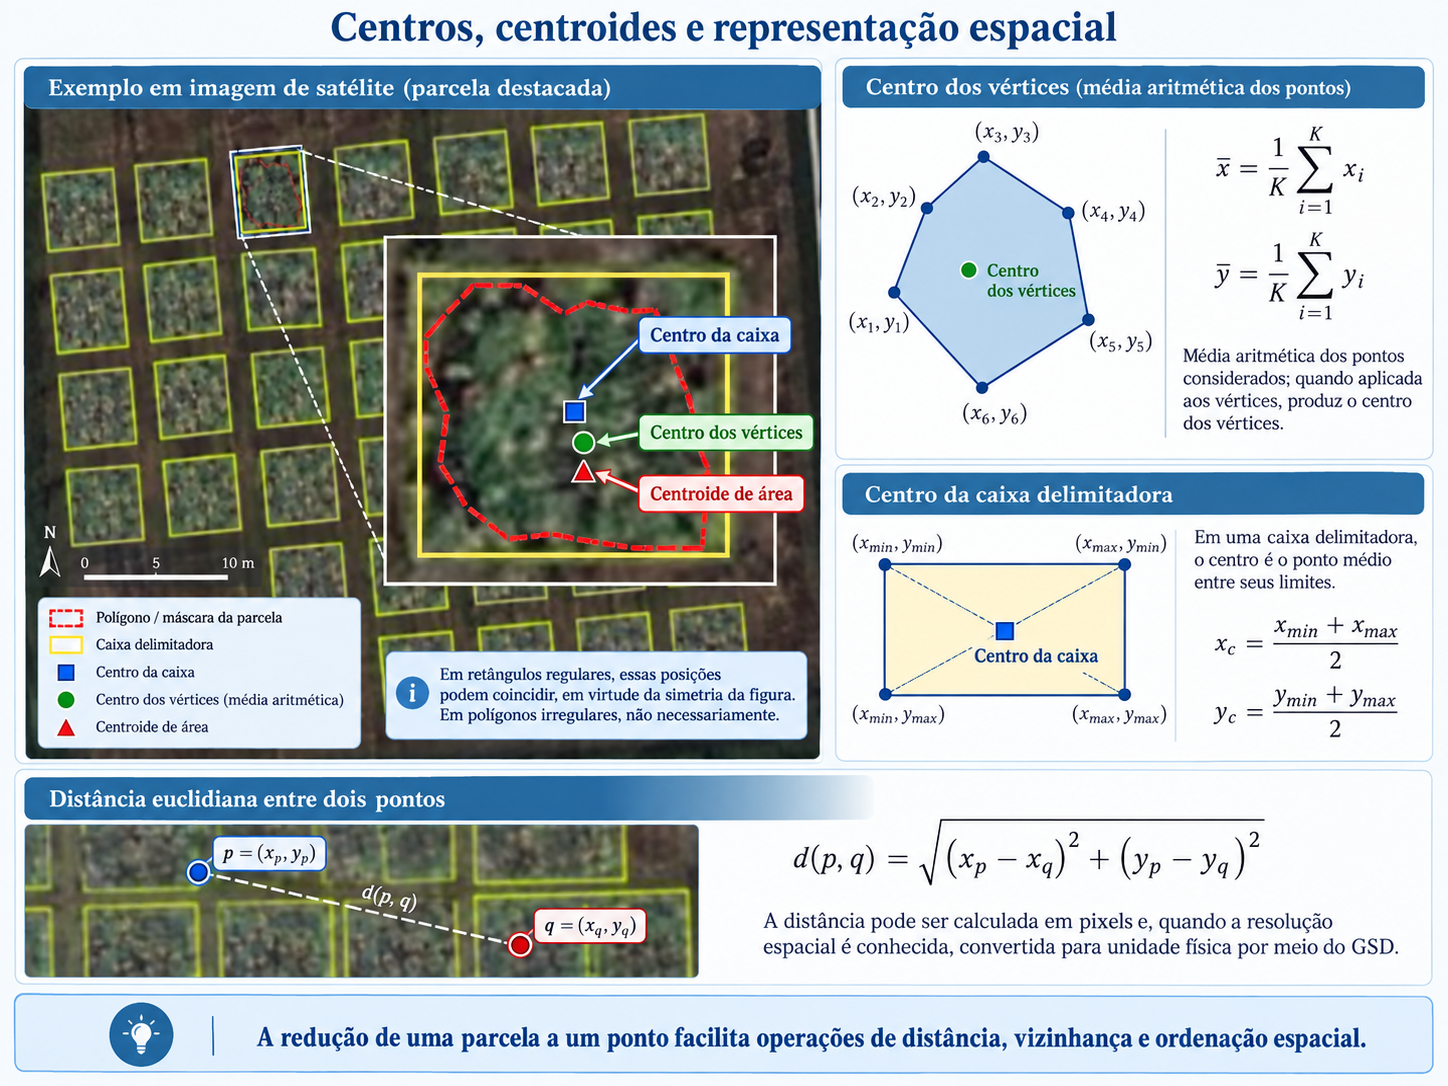
\includegraphics[width=0.9\textwidth]{figuras/figura07.png}
  \caption{Representa\c{c}\~ao de centros, centr\'oides e dist\^ancia euclidiana aplicados \`a localiza\c{c}\~ao espacial de parcelas experimentais em imagem orbital.}
  \label{fig:centros-centroides}
  \fonte{Elaborado pelo autor (2026).}
\end{figure}

Essa dist\^ancia pode ser calculada inicialmente em pixels e, quando a resolu\c{c}\~ao espacial \'e conhecida, convertida para unidade f\'isica por meio do GSD.

No sistema desenvolvido, medidas de dist\^ancia entre centros fazem parte das informa\c{c}\~oes utilizadas para avaliar a localiza\c{c}\~ao das detec\c{c}\~oes em rela\c{c}\~ao \`as anota\c{c}\~oes de refer\^encia.

\section{Organiza\c{c}\~ao espacial e estruturas em grade}
\label{sec:organizacao-espacial-grade}

A apar\^encia visual n\~ao \'e a \'unica fonte de informa\c{c}\~ao dispon\'ivel em um experimento agr\'icola. A disposi\c{c}\~ao planejada das parcelas tamb\'em estabelece rela\c{c}\~oes de posi\c{c}\~ao e vizinhan\c{c}a que podem ser utilizadas para interpretar as detec\c{c}\~oes produzidas a partir da imagem.

Em uma configura\c{c}\~ao organizada predominantemente por linhas e colunas, \'e poss\'ivel observar rela\c{c}\~oes entre posi\c{c}\~oes consecutivas, espa\c{c}amentos e alinhamentos. Essas regularidades podem fornecer informa\c{c}\~oes complementares quando se deseja estabelecer uma correspond\^encia entre objetos observados e posi\c{c}\~oes previstas.

\citet{mardanisamani2021} utiliza, por exemplo, a estrutura conhecida do experimento como ponto de partida para localizar as parcelas em ortomosaicos, refinando posteriormente a posi\c{c}\~ao da grade com base nas informa\c{c}\~oes da imagem. Este trabalho tenta demonstrar que a organiza\c{c}\~ao conhecida do campo, pode ser incorporada ao processo de localiza\c{c}\~ao, sem depender exclusivamente da an\'alise isolada de cada regi\~ao.

No problema investigado no escopo desta pesquisa, essa distin\c{c}\~ao se torna relevante quando uma parcela esperada n\~ao produz uma detec\c{c}\~ao. Se existem $N$ posi\c{c}\~oes previstas na organiza\c{c}\~ao experimental, mas apenas $N-K$ objetos s\~ao observados, o conjunto de detec\c{c}\~oes n\~ao representa integralmente a estrutura do experimento. Isso n\~ao significa que uma posi\c{c}\~ao ausente possa ser automaticamente reconstru\'ida apenas pela regularidade da grade. A infer\^encia de posi\c{c}\~oes faltantes constitui um problema adicional que precisa ser investigado e validado.

O interesse est\'a, portanto, em analisar de que maneira dist\^ancias, rela\c{c}\~oes de vizinhan\c{c}a, orienta\c{c}\~ao e conhecimento do croqui podem complementar a informa\c{c}\~ao visual. No projeto, essa dire\c{c}\~ao foi explorada por uma proposta referida como \textit{\textbf{Grid Completion}}, que consistia em estimar a dist\^ancia t\'ipica entre centros de parcelas vizinhas e, a partir dela, projetar as linhas e colunas da grade, de modo a ordenar as parcelas e estimar as posi\c{c}\~oes sem detec\c{c}\~ao correspondente.

\section{Informa\c{c}\~ao visual incompleta e posi\c{c}\~oes experimentais ausentes}
\label{sec:informacao-visual-incompleta}

A aus\^encia de evid\^encia visual e a inexist\^encia de uma posi\c{c}\~ao experimental representam situa\c{c}\~oes distintas. Uma parcela pode existir no planejamento do ensaio e, ainda assim, n\~ao produzir uma regi\~ao visual que um detector seja capaz de reconhecer. Nessa situa\c{c}\~ao, aquela posi\c{c}\~ao pode permanecer sem detec\c{c}\~ao correspondente, mesmo que a quantidade total de objetos preditos coincida com a de posi\c{c}\~oes previstas, pois detec\c{c}\~oes esp\'urias, isto \'e, predi\c{c}\~oes que n\~ao correspondem a nenhuma parcela, podem compensar numericamente as aus\^encias.

Essa diferen\c{c}a pode interferir principalmente em procedimentos de ordena\c{c}\~ao. Considere uma sequ\^encia de posi\c{c}\~oes $P_1, P_2, \ldots, P_N$. Se uma das posi\c{c}\~oes intermedi\'arias n\~ao possuir uma detec\c{c}\~ao associada e o algoritmo simplesmente ordenar os objetos observados de maneira consecutiva, as detec\c{c}\~oes posteriores poder\~ao ser associadas a identificadores incorretos. O problema passa, portanto, de uma tarefa exclusivamente visual para uma tarefa de correspond\^encia entre duas representa\c{c}\~oes: o conjunto de objetos observados e o conjunto de posi\c{c}\~oes previstas.

\begin{figure}[htb]
  \centering
  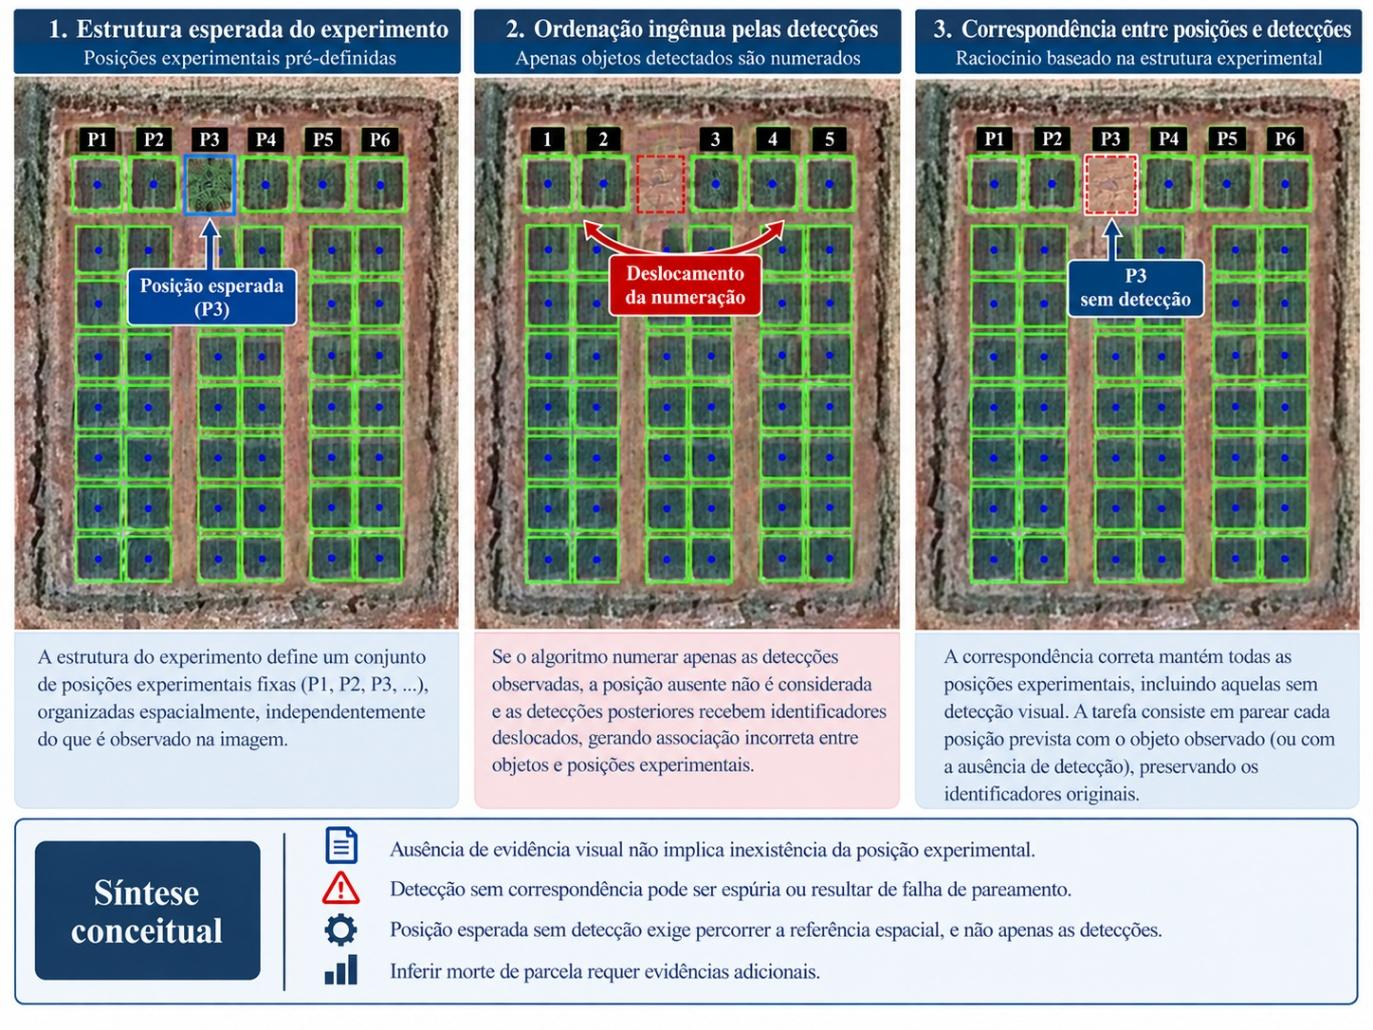
\includegraphics[width=0.95\textwidth]{figuras/figura08.jpg}
  \caption{Exemplo de deslocamento da numera\c{c}\~ao causado pela aus\^encia de detec\c{c}\~ao em uma posi\c{c}\~ao experimental.}
  \label{fig:deslocamento-numeracao}
  \fonte{Elaborado pelo autor (2026).}
\end{figure}

Conv\'em explicitar, neste ponto, que a afirma\c{c}\~ao de que uma parcela est\'a ausente ou morta, envolve uma cadeia de infer\^encias cujos elos dependem de evid\^encias pr\'oprias. Um objeto detectado que n\~ao encontra correspond\^encia em uma refer\^encia \'e o resultado de um procedimento de associa\c{c}\~ao, e pode decorrer de detec\c{c}\~ao esp\'uria, de cobertura parcial da refer\^encia ou de falha de pareamento. Um identificador da refer\^encia sem detec\c{c}\~ao associada \'e informa\c{c}\~ao de sentido oposto, e exige que o procedimento percorra a refer\^encia, e n\~ao apenas as detec\c{c}\~oes.

Uma posi\c{c}\~ao esperada sem evid\^encia visual \'e uma afirma\c{c}\~ao sobre o delineamento experimental, que pressup\~oe conhecimento da estrutura esperada. E a morte de uma parcela \'e uma afirma\c{c}\~ao agron\^omica, que pressup\~oe, al\'em da aus\^encia de evid\^encia visual, que essa aus\^encia n\~ao decorra de limita\c{c}\~ao do sensor, de oclus\~ao, de est\'agio fenol\'ogico ou de falha do detector. A passagem de um n\'ivel ao seguinte n\~ao \'e autom\'atica. Essa distin\c{c}\~ao orienta o projeto, contudo, o tratamento de posi\c{c}\~oes ausentes ainda n\~ao foi completamente sanado.

\section{Mapas de confian\c{c}a e representa\c{c}\~oes gaussianas}
\label{sec:mapas-confianca}

A detec\c{c}\~ao por caixas ou m\'ascaras n\~ao \'e a \'unica maneira de representar objetos em uma imagem. Em problemas de contagem e localiza\c{c}\~ao de objetos densamente distribu\'idos, tamb\'em podem ser empregados mapas cont\'inuos nos quais a posi\c{c}\~ao dos objetos \'e codificada espacialmente.

Uma maneira de construir essa representa\c{c}\~ao consiste em associar uma resposta gaussiana ao centro de cada objeto anotado. Um n\'ucleo gaussiano \'e uma fun\c{c}\~ao que atinge valor m\'aximo em um ponto central e decai suavemente \`a medida que a dist\^ancia a esse ponto aumenta, com a taxa desse decaimento controlada por um par\^ametro de dispers\~ao. Uma constru\c{c}\~ao poss\'ivel, a partir de $P$ posi\c{c}\~oes anotadas $(x_i, y_i)$, expressa-se como:

\begin{equation}
  F(x,y) = \sum_{i=1}^{P} \exp\left(-\frac{(x-x_i)^2 + (y-y_i)^2}{2\sigma^2}\right)
  \label{eq:mapa-confianca}
\end{equation}

em que $(x,y)$ \'e uma posi\c{c}\~ao qualquer do mapa, $(x_i, y_i)$ \'e a posi\c{c}\~ao do objeto $i$ e $\sigma$ controla a dispers\~ao espacial da resposta em torno dessa posi\c{c}\~ao.

\begin{figure}[htb]
  \centering
  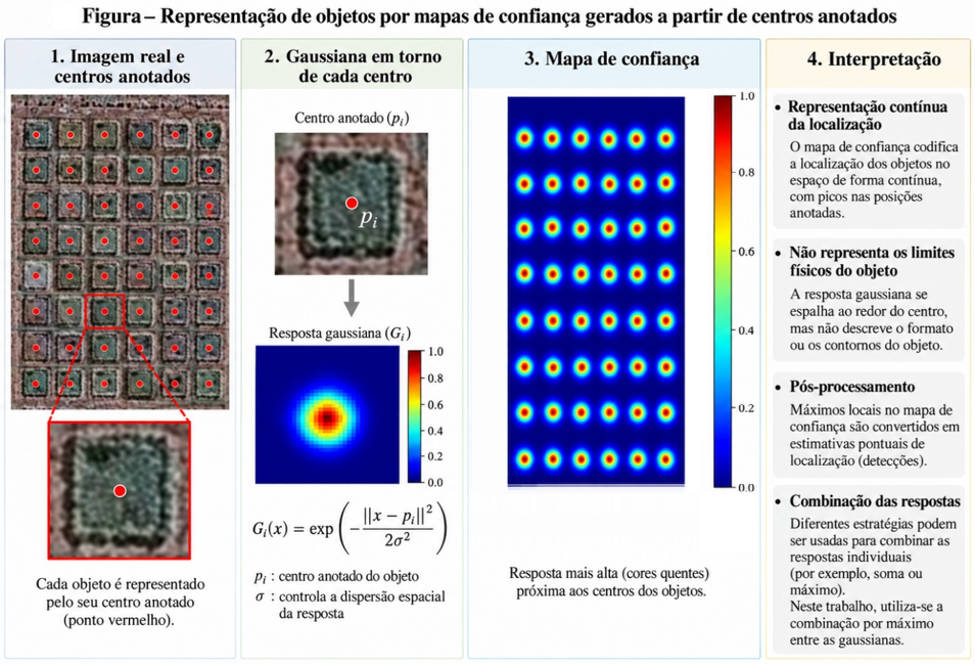
\includegraphics[width=0.9\textwidth]{figuras/figura09.png}
  \caption{Constru\c{c}\~ao de mapas de confian\c{c}a a partir de centros anotados em imagem real de parcelas experimentais.}
  \label{fig:mapas-confianca}
  \fonte{Elaborado pelo autor (2026).}
\end{figure}

Essa soma \'e uma entre outras formas poss\'iveis de combinar as respostas individuais. A implementa\c{c}\~ao do projeto n\~ao a utiliza diretamente, alternativamente, ela combina as respostas pelo valor m\'aximo em cada ponto. A escolha entre uma e outra altera o significado do mapa resultante, especialmente em regi\~oes densas, e a formula\c{c}\~ao supracitada n\~ao deve ser interpretada como descri\c{c}\~ao do procedimento local.

A representa\c{c}\~ao n\~ao delimita os limites f\'isicos do objeto. O mapa fornece uma indica\c{c}\~ao cont\'inua da intensidade da resposta associada \`a localiza\c{c}\~ao dos objetos; na implementa\c{c}\~ao, esses valores s\~ao amostrados em uma grade de pixels e utilizados para produzir estimativas pontuais por p\'os-processamento. Esses valores n\~ao constituem probabilidades calibradas pelo simples fato de serem designados como confian\c{c}a, e sua soma n\~ao corresponde necessariamente a uma contagem de objetos.

\citet{arruda2022} utilizaram essa ideia no contexto de contagem e localiza\c{c}\~ao de objetos em cen\'arios de elevada densidade, combinando enriquecimento dos mapas de caracter\'isticas com refinamento multiest\'agio de mapas de confian\c{c}a, avaliado em conjuntos de imagens de \'arvores e ve\'iculos. Essa abordagem \'e conceitualmente diferente da previs\~ao de uma caixa delimitadora, pois o objeto \'e representado principalmente por sua ocorr\^encia espacial, o que motivou sua considera\c{c}\~ao no desenvolvimento do projeto, dado o interesse em trabalhar com centros e com a localiza\c{c}\~ao de objetos distribu\'idos espacialmente.

\section{\textit{MultiStageRefinementNet}}
\label{sec:multistagerefinementnet}

\citet{arruda2022} prop\~oe uma abordagem para contagem e localiza\c{c}\~ao de objetos densamente distribu\'idos, baseada em redes neurais convolucionais e refinamento sucessivo de mapas de confian\c{c}a. Redes neurais convolucionais s\~ao arquiteturas que aplicam filtros aprendidos sobre regi\~oes locais da imagem, compondo representa\c{c}\~oes progressivamente mais abstratas a partir de padr\~oes visuais elementares.

A arquitetura proposta organiza-se em tr\^es componentes. Um extrator de caracter\'isticas reduz a resolu\c{c}\~ao espacial da imagem de entrada e produz uma representa\c{c}\~ao intermedi\'aria. Um m\'odulo de agrega\c{c}\~ao em pir\^amide, denominado \textit{\textbf{Pyramid Pooling Module}} \citep{zhao2017}, combina informa\c{c}\~oes obtidas por agrupamento em diferentes escalas, incorporando \`a representa\c{c}\~ao contexto de extens\~oes variadas. Uma sequ\^encia de est\'agios de refinamento, produz mapas de confian\c{c}a sucessivos, em que cada est\'agio recebe a sa\'ida do m\'odulo de agrega\c{c}\~ao e, a partir do segundo, o mapa produzido pelo est\'agio anterior.

Os alvos de treinamento de cada est\'agio s\~ao constru\'idos com valores decrescentes de $\sigma$, de modo que os est\'agios iniciais aprendam uma localiza\c{c}\~ao aproximada e os finais a refinem. Em vez de produzir uma \'unica estimativa espacial e encerr\'a-la, os est\'agios sucessivos procuram refinar as respostas geradas, favorecendo a localiza\c{c}\~ao de objetos em regi\~oes densas. A sa\'ida da rede \'e um mapa de confian\c{c}a representado em uma grade de pixels; as posi\c{c}\~oes dos objetos s\~ao obtidas em etapa posterior, pela identifica\c{c}\~ao de m\'aximos locais.

\'E importante diferenciar essa arquitetura, tal como descrita na publica\c{c}\~ao, da implementa\c{c}\~ao incorporada ao projeto. No m\'etodo publicado, o extrator de caracter\'isticas baseia-se na \textit{\textbf{VGG19}} \citep{simonyan2015}, arquitetura convolucional profunda de camadas sequenciais amplamente utilizada como extrator pr\'e-treinado. Na implementa\c{c}\~ao do projeto, a configura\c{c}\~ao padr\~ao utiliza um extrator simplificado, inspirado na VGG19 e sem pesos pr\'e-treinados, e houve tamb\'em treinamentos com essa arquitetura pr\'e-treinada.

A denomina\c{c}\~ao \textit{MultiStageRefinementNet} \'e a empregada no c\'odigo do projeto, e n\~ao necessariamente a utilizada na publica\c{c}\~ao de refer\^encia. A implementa\c{c}\~ao local foi desenvolvida em \textit{TensorFlow} e \textit{Keras} e permaneceu separada do fluxo principal, desenvolvido em \textit{PyTorch}.

No contexto desta pesquisa, essa abordagem constitui uma fam\'ilia metodol\'ogica diferente da detec\c{c}\~ao e da segmenta\c{c}\~ao baseadas em YOLO, pois privilegia a representa\c{c}\~ao espacial baseada em pontos e mapas de confian\c{c}a, sem delimitar a extens\~ao dos objetos.

\section{Classifica\c{c}\~ao de imagens e \textit{EfficientNet}}
\label{sec:classificacao-efficientnet}

A classifica\c{c}\~ao de imagens associa uma entrada visual a uma categoria global. Essa tarefa difere da detec\c{c}\~ao e da segmenta\c{c}\~ao porque n\~ao exige localizar os objetos respons\'aveis pela decis\~ao: a sa\'ida \'e um r\'otulo atribu\'ido \`a imagem como um todo.

A fam\'ilia \textit{EfficientNet} foi proposta por \citet{tan2019} a partir da investiga\c{c}\~ao do escalonamento de redes neurais convolucionais. Os autores observam que aumentar isoladamente a profundidade da rede, sua largura ou a resolu\c{c}\~ao da entrada nem sempre produz a melhor rela\c{c}\~ao entre desempenho e custo computacional, e prop\~oem um esquema de escalonamento composto, no qual essas tr\^es dimens\~oes s\~ao ampliadas conjuntamente segundo coeficientes relacionados por um fator \'unico.

A \textit{EfficientNet-B0} corresponde ao modelo de menor escala dessa fam\'ilia, obtido por busca de arquitetura, e serve de base a partir da qual as demais variantes s\~ao constru\'idas pela aplica\c{c}\~ao daquele esquema de escalonamento. Redes dessa fam\'ilia s\~ao frequentemente empregadas como extratores de caracter\'isticas pr\'e-treinados, com substitui\c{c}\~ao da camada final para adapta\c{c}\~ao a uma tarefa espec\'ifica.

Neste trabalho, uma \textit{EfficientNet-B0} foi empregada como componente auxiliar para classifica\c{c}\~ao bin\'aria da dificuldade operacional das imagens, a partir de r\'otulos derivados do comportamento de um detector. A classifica\c{c}\~ao n\~ao constitui o n\'ucleo do problema cient\'ifico da pesquisa e, por isso, a fundamenta\c{c}\~ao conceitual necess\'aria para esse componente \'e limitada.

\section{M\'etricas de avalia\c{c}\~ao}
\label{sec:metricas-avaliacao}

A avalia\c{c}\~ao de sistemas de detec\c{c}\~ao, segmenta\c{c}\~ao e localiza\c{c}\~ao exige medidas que representem diferentes aspectos do erro. Uma \'unica m\'etrica raramente caracteriza integralmente o desempenho de um modelo.

\textbf{\textit{Intersection over Union} (IoU):} Essa m\'etrica mede o grau de sobreposi\c{c}\~ao entre duas regi\~oes, comparando a \'area compartilhada com a \'area total ocupada por ambas. Corresponde ao \'indice de Jaccard aplicado \`as regi\~oes. Para uma regi\~ao predita $A$ e uma regi\~ao de refer\^encia $B$:

\begin{equation}
  \mathit{IoU}(A,B) = \frac{|A \cap B|}{|A \cup B|}
  \label{eq:iou}
\end{equation}

O resultado varia entre 0 e 1. Valores mais pr\'oximos de 1 indicam maior sobreposi\c{c}\~ao. A \textit{IoU} pode ser calculada tanto sobre caixas delimitadoras quanto sobre m\'ascaras, e sua interpreta\c{c}\~ao depende da representa\c{c}\~ao utilizada e do limiar definido para considerar uma correspond\^encia v\'alida.

Precis\~ao (\textit{Precision}): Expressa a propor\c{c}\~ao de detec\c{c}\~oes consideradas corretas entre todas as detec\c{c}\~oes produzidas pelo modelo:

\begin{equation}
  \mathit{Precision} = \frac{TP}{TP + FP}
  \label{eq:precision}
\end{equation}

em que $TP$ representa verdadeiros positivos e $FP$ representa falsos positivos.

Recall: Expressa a propor\c{c}\~ao dos objetos de refer\^encia que receberam uma detec\c{c}\~ao considerada correspondente:

\begin{equation}
  \mathit{Recall} = \frac{TP}{TP + FN}
  \label{eq:recall}
\end{equation}

em que $FN$ representa falsos negativos.

F1-score (F1): Combina precis\~ao e \textit{recall} por meio da m\'edia harm\^onica:

\begin{equation}
  F_1 = 2\,\frac{\mathit{Precision} \cdot \mathit{Recall}}{\mathit{Precision} + \mathit{Recall}}
  \label{eq:f1}
\end{equation}

\begin{figure}[htb]
  \centering
  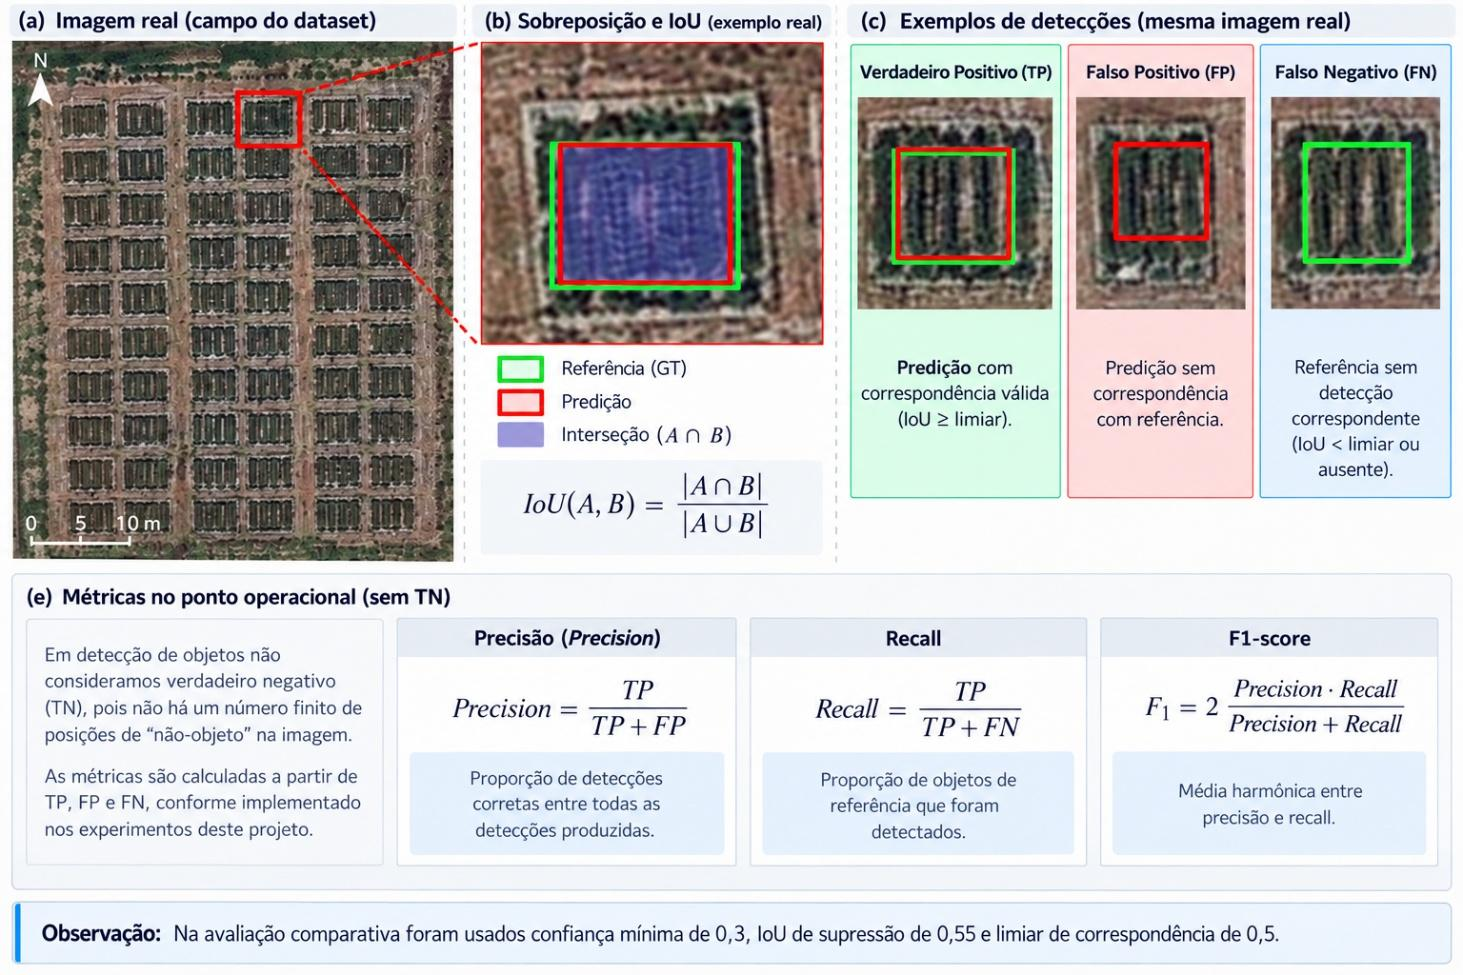
\includegraphics[width=0.95\textwidth]{figuras/figura10.jpg}
  \caption{Ilustra\c{c}\~ao conceitual de IoU, verdadeiro positivo, falso positivo, falso negativo, precis\~ao, recall e F1-score em detec\c{c}\~ao de parcelas experimentais.}
  \label{fig:iou-conceitual}
  \fonte{Elaborado pelo autor (2026).}
\end{figure}

Esse valor permite observar conjuntamente o efeito de falsos positivos e falsos negativos, embora n\~ao substitua a an\'alise individual de precis\~ao e \textit{recall}.

No que se refere em agrega\c{c}\~ao das medidas: Em conjuntos formados por v\'arias imagens, precis\~ao, \textit{recall} e \textit{F1} podem ser apresentados de maneiras distintas. As medidas globais s\~ao obtidas a partir das contagens acumuladas de verdadeiros positivos, falsos positivos e falsos negativos de todas as imagens consideradas. Alternativamente, podem ser calculadas m\'etricas individualmente para cada imagem e posteriormente obtida sua m\'edia, atribuindo o mesmo peso a cada imagem.

Essas formas de agrega\c{c}\~ao n\~ao s\~ao intercambi\'aveis: na agrega\c{c}\~ao global, os denominadores tamb\'em diferem entre as m\'etricas: a precis\~ao depende de $TP+FP$, enquanto o \textit{recall} depende de $TP+FN$. O F1 global \'e calculado a partir da precis\~ao e do \textit{recall} globais e, portanto, n\~ao corresponde necessariamente \`a m\'edia dos F1 obtidos individualmente por imagem.

Distin\c{c}\~ao semelhante ocorre para a \textit{IoU}: na avalia\c{c}\~ao utilizada neste projeto, s\~ao reportadas uma m\'edia da sobreposi\c{c}\~ao por imagem e uma m\'edia ponderada pelo n\'umero de correspond\^encias. A primeira atribui o mesmo peso \`as imagens consideradas, enquanto a segunda atribui maior peso \`as imagens com maior n\'umero de pares v\'alidos.

\textit{Average Precision e Mean Average Precision}: A \textit{Average Precision (AP)} resume a rela\c{c}\~ao entre precis\~ao e \textit{recall}, ao longo de diferentes n\'iveis de confian\c{c}a das predi\c{c}\~oes, condensando em um \'unico valor: a curva precis\~ao--recall. Protocolos como o \textit{PASCAL VOC} contribu\'iram para consolidar o uso dessa medida na avalia\c{c}\~ao de detectores \citep{everingham2010}.

Para um crit\'erio de sobreposi\c{c}\~ao fixado e $C$ classes, a m\'edia entre as AP das classes pode ser expressa por:

\begin{equation}
  mAP = \frac{1}{C}\sum_{c=1}^{C} AP_c
  \label{eq:map}
\end{equation}

Quando existe apenas uma classe, a m\'edia entre classes coincide numericamente com a \textit{AP} dessa classe para o mesmo crit\'erio de avalia\c{c}\~ao.

A avalia\c{c}\~ao pode ainda considerar diferentes limiares de \textit{IoU}: o \textbf{\textit{COCO}} \'e um conjunto p\'ublico de dados para reconhecimento de objetos que inclui tarefas de detec\c{c}\~ao e segmenta\c{c}\~ao \citep{lin2014}. Em seu protocolo oficial, uma das medidas sintetiza o desempenho em limiares de IoU entre 0,50 e 0,95, em incrementos de 0,05 \citep{cocoapi}. Esse crit\'erio \'e mais restritivo que uma avalia\c{c}\~ao realizada somente em \textit{IoU} igual a 0,50.

\'E necess\'ario distinguir duas varia\c{c}\~oes independentes: a primeira corresponde \`a confian\c{c}a das predi\c{c}\~oes, utilizada na constru\c{c}\~ao da curva precis\~ao--recall e, consequentemente, da \textit{AP}. A segunda corresponde ao crit\'erio de sobreposi\c{c}\~ao utilizado para determinar a qualidade espacial da detec\c{c}\~ao. Assim, \textbf{\textit{mAP@0,5}} e \textbf{\textit{mAP@0,5:0,95}} n\~ao representam apenas valores calculados em diferentes limiares de confian\c{c}a: diferem tamb\'em pelo conjunto de limiares de \textit{IoU} considerados.

Nos experimentos deste projeto s\~ao reportadas as duas medidas. Elas s\~ao obtidas por uma rotina de avalia\c{c}\~ao distinta da que calcula as m\'etricas por imagem em um ponto operacional; por isso, \textbf{\textit{mAP}}, precis\~ao global, \textit{recall, F1} e \textit{IoU} s\~ao interpretados de acordo com o protocolo que originou cada resultado.

Dist\^ancia entre centros: Quando o interesse inclui a qualidade da localiza\c{c}\~ao espacial, a dist\^ancia entre a posi\c{c}\~ao representativa de uma predi\c{c}\~ao e a posi\c{c}\~ao correspondente da refer\^encia fornece uma medida complementar \`a sobreposi\c{c}\~ao. Para dois pontos $p = (x_p, y_p)$ e $q = (x_q, y_q)$:

\begin{equation}
  d(p,q) = \sqrt{(x_p - x_q)^2 + (y_p - y_q)^2}
  \label{eq:distancia-centros-metrica}
\end{equation}

\begin{figure}[htb]
  \centering
  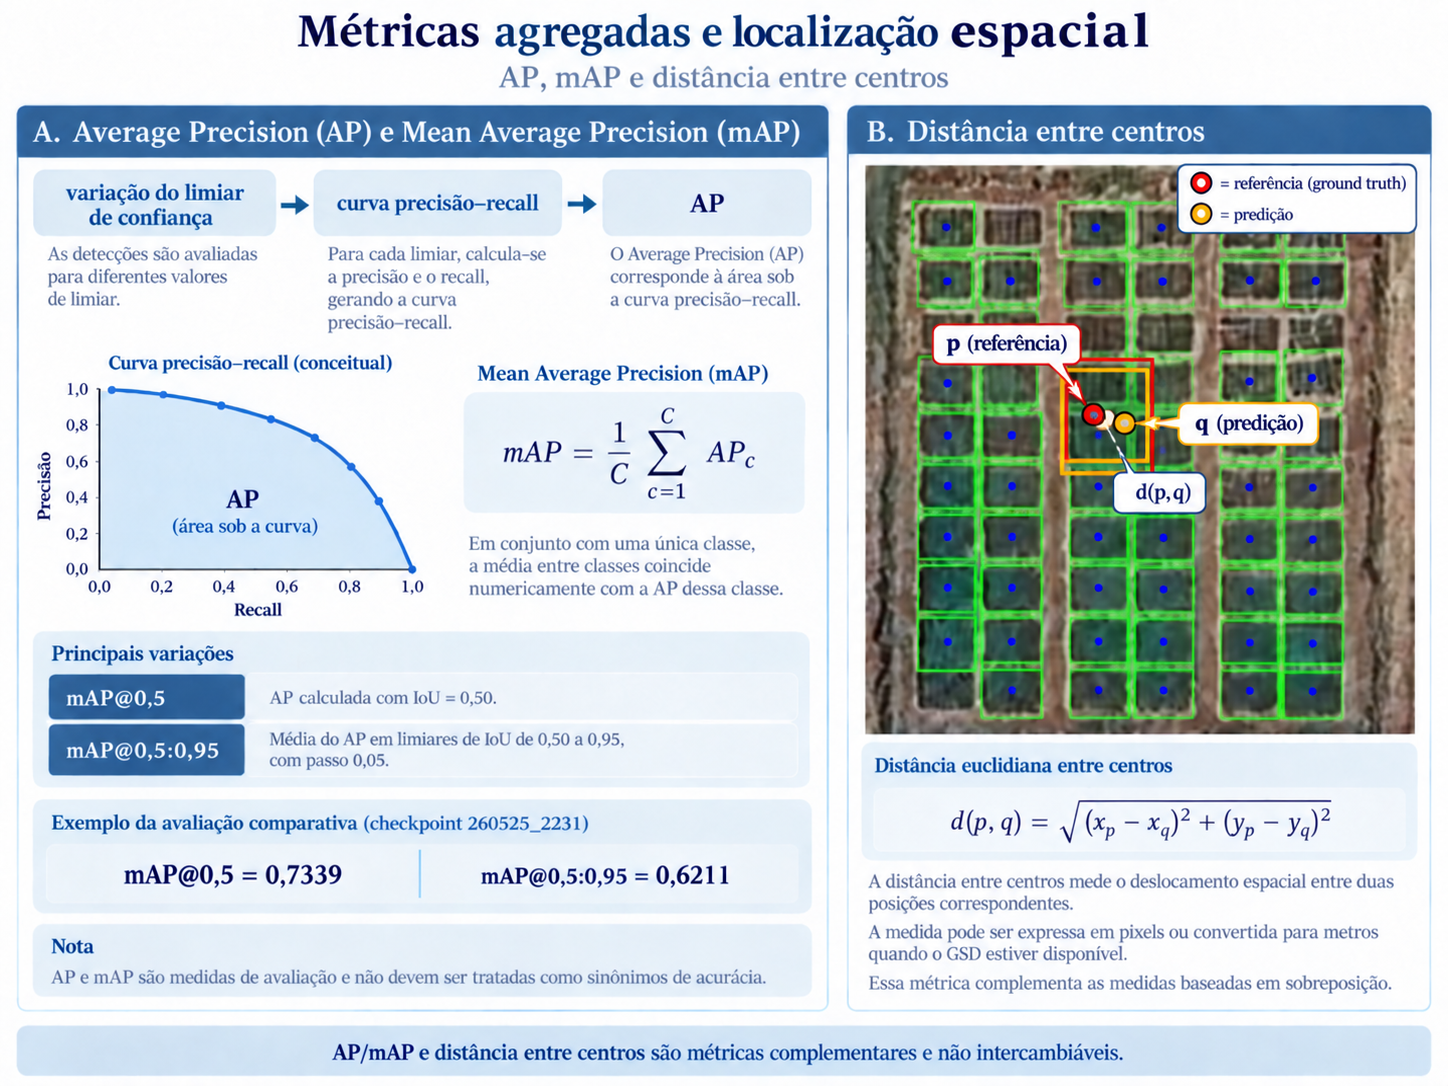
\includegraphics[width=0.9\textwidth]{figuras/figura11.png}
  \caption{Rela\c{c}\~ao entre AP, mAP e dist\^ancia entre centros na avalia\c{c}\~ao de detec\c{c}\~ao e localiza\c{c}\~ao espacial.}
  \label{fig:ap-map-distancia}
  \fonte{Elaborado pelo autor (2026).}
\end{figure}

A dist\^ancia \'e expressa em pixels, com a convers\~ao para unidades f\'isicas descrita na Se\c{c}\~ao~\ref{sec:resolucao-espacial}. Essa medida \'e relevante neste projeto porque uma parcela pode apresentar correspond\^encia visual satisfat\'oria e, ainda assim, possuir deslocamento espacial capaz de interferir nas etapas posteriores de associa\c{c}\~ao e organiza\c{c}\~ao das parcelas.

\section{Correspond\^encia entre previs\~oes e anota\c{c}\~oes}
\label{sec:correspondencia-previsoes}

Para calcular m\'etricas baseadas em verdadeiros positivos, falsos positivos e falsos negativos, \'e necess\'ario estabelecer quais predi\c{c}\~oes correspondem a quais anota\c{c}\~oes de refer\^encia.

Essa associa\c{c}\~ao pode ser realizada segundo diferentes crit\'erios. A \textit{Intersection over Union} (IoU) \'e empregada quando se deseja avaliar a sobreposi\c{c}\~ao entre regi\~oes, enquanto a dist\^ancia entre centros pode ser utilizada quando o interesse recai sobre a proximidade espacial das posi\c{c}\~oes representativas. No sistema desenvolvido existem procedimentos baseados nesses dois tipos de informa\c{c}\~ao. Na avalia\c{c}\~ao comparativa desta pesquisa, entretanto, as diferentes representa\c{c}\~oes de sa\'ida s\~ao convertidas para pol\'igonos e a associa\c{c}\~ao entre predi\c{c}\~oes e refer\^encias \'e determinada a partir da \textit{IoU}.

Quando cada predi\c{c}\~ao e cada anota\c{c}\~ao devem participar de no m\'aximo uma correspond\^encia, o problema assume uma estrutura de pareamento um-para-um. Os limiares utilizados para aceitar ou rejeitar uma associa\c{c}\~ao pertencem \`a configura\c{c}\~ao experimental e, portanto, n\~ao como valores te\'oricos universais.

Conv\'em distinguir dois problemas de correspond\^encia presentes neste trabalho. No primeiro, predi\c{c}\~oes s\~ao comparadas \`as anota\c{c}\~oes de refer\^encia da mesma imagem, com a finalidade de determinar acertos e erros de detec\c{c}\~ao. No segundo, objetos detectados em uma nova imagem de um campo s\~ao associados a uma refer\^encia espacial previamente numerada pelo operador, com o objetivo de transferir os identificadores das parcelas entre imagens. Essa refer\^encia \'e constru\'ida a partir das detec\c{c}\~oes numeradas e armazenada pelo sistema, n\~ao correspondendo a uma importa\c{c}\~ao autom\'atica do croqui agron\^omico.

Quando se busca minimizar conjuntamente o custo das correspond\^encias, a associa\c{c}\~ao pode ser formulada como um problema de atribui\c{c}\~ao linear, resolvido classicamente pelo m\'etodo h\'ungaro \citep{kuhn1955}. Nessa formula\c{c}\~ao, procura-se um conjunto de pares que minimize o custo total, impedindo que um mesmo elemento seja reutilizado em mais de uma correspond\^encia. Em matrizes retangulares, conjuntos de tamanhos diferentes permitem que elementos do conjunto maior perman\c{c}am sem par \citep{scipy}. A obten\c{c}\~ao da solu\c{c}\~ao de menor custo para a matriz constru\'ida n\~ao implica, entretanto, que os pares encontrados correspondam necessariamente \`as identidades corretas no delineamento experimental.

O segundo problema apresenta ainda uma dificuldade geom\'etrica: os conjuntos de pontos obtidos em imagens distintas de um mesmo campo podem apresentar diferen\c{c}as de posi\c{c}\~ao, escala e orienta\c{c}\~ao. O registro de conjuntos de pontos busca reduzir essas diferen\c{c}as antes da associa\c{c}\~ao. O m\'etodo \textit{Coherent Point Drift} (\textit{CPD}) \citep{myronenko2010} formula esse registro probabilisticamente, tratando os pontos de um conjunto como centr\'oides de uma mistura de distribui\c{c}\~oes gaussianas ajustada ao outro conjunto.

No procedimento implementado, o registro por \textit{CPD} \'e aplicado aos centros das detec\c{c}\~oes para aproximar o conjunto correspondente \`a nova imagem da refer\^encia espacial. A determina\c{c}\~ao das identidades ocorre posteriormente, por meio de uma fun\c{c}\~ao de custo e de uma atribui\c{c}\~ao um-para-um. Dessa forma, registro geom\'etrico e atribui\c{c}\~ao de identidade constituem etapas distintas: o primeiro aproxima espacialmente os conjuntos; o segundo determina quais elementos ser\~ao considerados correspondentes.

\section{Generaliza\c{c}\~ao e depend\^encia entre amostras}
\label{sec:generalizacao-dependencia}

O treinamento de um modelo de aprendizado supervisionado procura ajustar seus par\^ametros a partir de exemplos dispon\'iveis, mas o interesse cient\'ifico normalmente est\'a em seu comportamento sobre observa\c{c}\~oes que n\~ao participaram desse processo.

Por essa raz\~ao, os dados costumam ser separados em conjuntos com fun\c{c}\~oes distintas. O conjunto de treinamento \'e utilizado para atualizar os par\^ametros do modelo. O conjunto de valida\c{c}\~ao pode ser utilizado durante o desenvolvimento para sele\c{c}\~ao de configura\c{c}\~oes e acompanhamento do comportamento do treinamento. O conjunto de teste deve fornecer uma avalia\c{c}\~ao sobre dados preservados da etapa de ajuste.

\begin{figure}[htb]
  \centering
  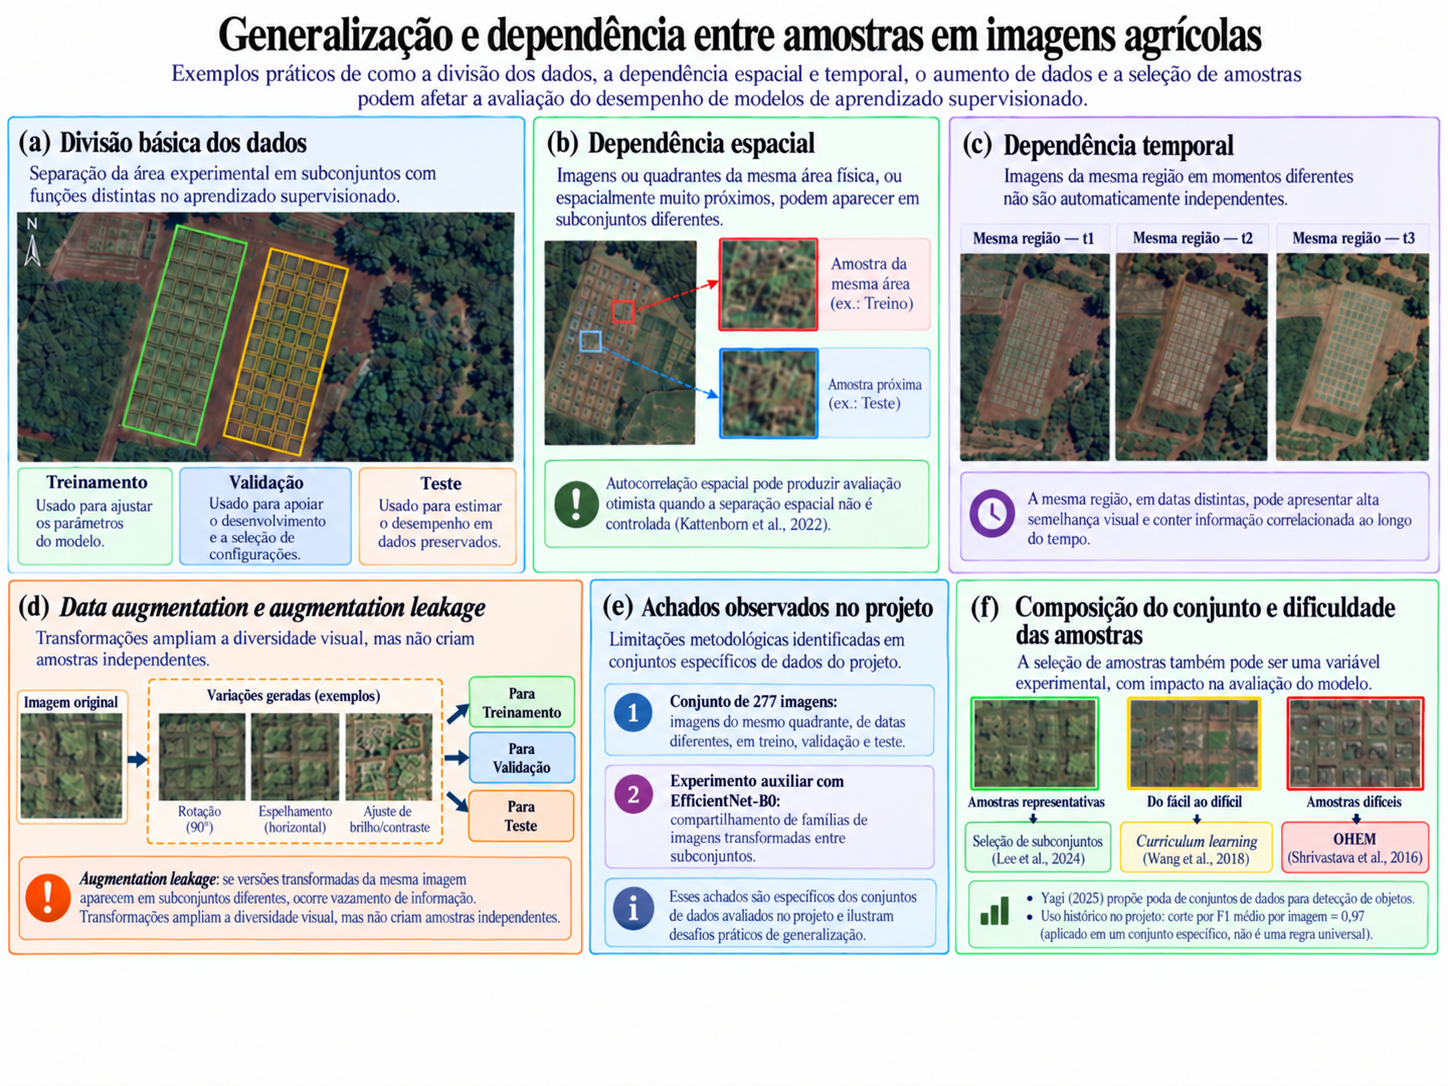
\includegraphics[width=0.95\textwidth]{figuras/figura12.png}
  \caption{Generaliza\c{c}\~ao, depend\^encia espacial e temporal, augmentation leakage e sele\c{c}\~ao de amostras no treinamento de modelos.}
  \label{fig:generalizacao-dependencia}
  \fonte{Elaborado pelo autor (2026).}
\end{figure}

A validade dessa avalia\c{c}\~ao depende n\~ao apenas de os arquivos terem nomes diferentes, mas tamb\'em do grau de independ\^encia entre as observa\c{c}\~oes. Em dados geoespaciais, imagens espacialmente pr\'oximas ou provenientes da mesma \'area podem compartilhar caracter\'isticas que tornam a tarefa de previs\~ao mais semelhante \`aquela observada no treinamento.

\citet{kattenborn2022} demonstram, em um problema de segmenta\c{c}\~ao com imagens de sensoriamento remoto, que a presen\c{c}a de amostras espacialmente autocorrelacionadas entre treinamento e valida\c{c}\~ao pode produzir avalia\c{c}\~oes mais otimistas do que aquelas obtidas quando a separa\c{c}\~ao espacial \'e considerada explicitamente.

Assim, quando imagens da mesma regi\~ao f\'isica aparecem em subconjuntos diferentes, n\~ao \'e poss\'ivel assumir automaticamente que o desempenho observado representa a capacidade de transfer\^encia para regi\~oes independentes. Isso tamb\'em n\~ao significa que o modelo necessariamente tenha memorizado a \'area. A conclus\~ao metodologicamente adequada \'e que a correla\c{c}\~ao entre as observa\c{c}\~oes reduz a independ\^encia da avalia\c{c}\~ao e limita a interpreta\c{c}\~ao das m\'etricas como estimativas de generaliza\c{c}\~ao espacial.

A depend\^encia entre observa\c{c}\~oes tamb\'em pode ocorrer no dom\'inio temporal. Imagens adquiridas na mesma regi\~ao em momentos distintos podem compartilhar padr\~oes de solo, organiza\c{c}\~ao das parcelas, limites f\'isicos e outras caracter\'isticas visuais. Quando essas observa\c{c}\~oes s\~ao distribu\'idas entre treinamento e teste, a interpreta\c{c}\~ao do desempenho deve considerar essa correla\c{c}\~ao.

O aumento de dados, \textit{data augmentation}, possui finalidade diferente. Trata-se da aplica\c{c}\~ao de transforma\c{c}\~oes \`as imagens dispon\'iveis, como rota\c{c}\~oes, espelhamentos, altera\c{c}\~oes de brilho ou outras perturba\c{c}\~oes, com o objetivo de ampliar a diversidade visual apresentada durante o treinamento sem exigir novas coletas.

Essas transforma\c{c}\~oes, entretanto, n\~ao produzem observa\c{c}\~oes independentes de sua imagem de origem. Imagens derivadas do mesmo original continuam compartilhando grande parte de seu conte\'udo. Quando derivados de uma mesma imagem s\~ao distribu\'idos entre treinamento e teste, ocorre uma forma de \textit{augmentation leakage}, pois o conjunto de teste passa a conter informa\c{c}\~ao fortemente relacionada a dados que tamb\'em participaram do treinamento.

A composi\c{c}\~ao do conjunto de treinamento tamb\'em pode ser tratada como vari\'avel experimental. Em detec\c{c}\~ao supervisionada, diferentes trabalhos utilizam dificuldade ou informatividade das amostras de formas distintas. O \textit{Online Hard Example Mining} prioriza exemplos dif\'iceis durante o treinamento de detectores \citep{shrivastava2016}. \citet{wang2018} organizam amostras segundo sua dificuldade em uma estrat\'egia de \textit{curriculum learning}. Em outra dire\c{c}\~ao, \citet{lee2024} investigam a sele\c{c}\~ao de subconjuntos representativos e diversos especificamente para detec\c{c}\~ao de objetos.

\citet{yagi2025}, em trabalho dispon\'ivel como \textit{preprint}, estende a discuss\~ao de \textit{dataset pruning} \`a detec\c{c}\~ao de objetos e prop\~oe o \textit{Variance-based Prediction Score}, calculado pela varia\c{c}\~ao, ao longo das \'epocas de treinamento, do \textit{IoU} ou da confian\c{c}a da predi\c{c}\~ao associada a cada objeto, com posterior agrega\c{c}\~ao das medidas dos objetos para o n\'ivel da imagem. Nesse \textit{score}, valores baixos correspondem a objetos detectados ou n\~ao detectados de forma consistente, e valores altos, a objetos de dificuldade intermedi\'aria; as imagens de menor escore s\~ao removidas. No \textit{PASCAL VOC}, a sele\c{c}\~ao por esse escore superou subconjuntos aleat\'orios de mesmo tamanho em todas as taxas de remo\c{c}\~ao avaliadas, mas permaneceu abaixo do conjunto completo. Em outro regime de aprendizagem, \citet{zhang2026} analisa, na aprendizagem contrastiva n\~ao supervisionada, pares de amostras de classes diferentes com alta similaridade e mostraram que a remo\c{c}\~ao ou o tratamento espec\'ifico desses pares pode melhorar a generaliza\c{c}\~ao. Esses trabalhos empregam tarefas, unidades de an\'alise e defini\c{c}\~oes de dificuldade distintas e n\~ao demonstram que exemplos dif\'iceis devam necessariamente ser exclu\'idos ou priorizados. Em conjunto, mostram que a contribui\c{c}\~ao das amostras depende do crit\'erio de sele\c{c}\~ao e que a composi\c{c}\~ao do conjunto de treinamento pode ser investigada como parte do pr\'oprio problema de aprendizagem.

Quando a dificuldade de uma imagem \'e estimada a partir do desempenho de um modelo, deve-se ainda considerar a independ\^encia entre o modelo utilizado para produzir essa estimativa e a imagem avaliada. Se uma imagem tiver participado do ajuste do detector que posteriormente \'e utilizado para classific\'a-la como f\'acil ou dif\'icil, a medida poder\'a refletir parcialmente o contato pr\'evio do modelo com aquela observa\c{c}\~ao. Por essa raz\~ao, nesta pesquisa o crit\'erio de sele\c{c}\~ao ser\'a calculado em imagens que n\~ao participaram do treinamento do modelo que as avalia, e o efeito da sele\c{c}\~ao ser\'a medido em grupos de teste separados.

As compara\c{c}\~oes das propostas futuras, permitir\~ao investigar se altera\c{c}\~oes na composi\c{c}\~ao do conjunto de treinamento afetam a capacidade de generaliza\c{c}\~ao do detector. A proposta n\~ao pressup\~oe que remover imagens consideradas dif\'iceis produzir\'a melhora: o efeito poder\'a ser positivo, negativo ou inexistente, e dever\'a ser determinado experimentalmente.
